\documentclass[12pt]{article}

% ---------- Packages ----------
\usepackage[utf8]{inputenc}
\usepackage[T1]{fontenc}
\usepackage{geometry}
\geometry{margin=1in}
\usepackage{graphicx}
\usepackage{amsmath}
\usepackage{amssymb}
\usepackage{array}
\usepackage{booktabs}
\usepackage{enumitem}
\usepackage{hyperref}
\hypersetup{
    colorlinks=true,
    linkcolor=black,
    citecolor=black,
    urlcolor=blue,
}
\usepackage{longtable}
\usepackage{caption}
\usepackage{float}
\usepackage{setspace}
\graphicspath{{figures/}}

% ---------- Title Information ----------
\title{Architectural Design and Trade-Off Analysis of a Real-Time Ride-Sharing Platform Backend}
\author{Travis Holt}
\date{\today}

% Fill in course details
\newcommand{\courseName}{COMP 6231: Distributed Systems}
\newcommand{\assignmentName}{Assignment 1}
\newcommand{\instructorName}{Dr. Reza Mirsalari}
\newcommand{\studentId}{40351596}

\begin{document}

% ---------- Title Page ----------
\begin{titlepage}
    \centering
    \vspace*{2cm}
    {\LARGE \textbf{\courseName}}\\[0.5cm]
    {\Large \assignmentName}\\[1.5cm]
    {\Huge \textbf{Architectural Design and Trade-Off Analysis of a Real-Time Ride-Sharing Platform Backend}}\\[2cm]

    \vfill

    {\large
    \begin{tabular}{ll}
        Author: & Travis Holt \\
        Student ID: & \studentId \\
        Instructor: & \instructorName \\
        Date: & \today \\
    \end{tabular}
    }

    \vspace*{1cm}
\end{titlepage}

% \tableofcontents
% \newpage

% ---------- Introduction ----------
\section{Introduction}
\label{sec:introduction}

\subsection{Problem Statement}
"...architect the backend infrastructure of a real-time ride-sharing platform similar to Uber or Lyft, using principles
from distributed systems. Your task is to analyze and design a distributed backend
system that supports high availability, low latency, and data consistency under high
concurrency."

You must integrate and analyze the following core architectural components
\begin{itemize}
    \item Database Sharding (Hash-based, Range-based, or Consistent Hashing)
    \item Replication and Consistency Models (Eventual, Strong, Quorum-based)
    \item Load Balancing (Layer 4 vs. Layer 7)
\end{itemize}

\subsection{System Requirements}

\subsubsection{Functional Requirements}
\begin{itemize}
    \item Drivers broadcast live location and availability.
    \item Riders send trip requests that are matched with nearby drivers.
    \item The system supports live matching, route calculation, and payment processing.
    \item Data includes user accounts, trip histories, real-time GPS data, and pricing rules.
\end{itemize}

\subsubsection{Non-Functional Requirements}
\begin{itemize}
    \item Global scale support (multi-region architecture assumed).
    \item Sub-200ms latency for ride-matching response in 90\% of requests.
    \item High read/write throughput for hotspots (e.g., downtown during peak hours).
\end{itemize}

\subsection{Report Organization}
The proposed system is introduced graphically with a series of architecture diagrams with increasing granularity. Design considerations, trade-offs, and decisions are discussed subsequently. The report concludes with recommendations for implementing this system.


% ---------- System Architecture Overview ----------
\section{System Architecture Overview}
\label{sec:architecture-overview}

\subsection{System Diagrams}

\begin{figure}[H]
    \centering
    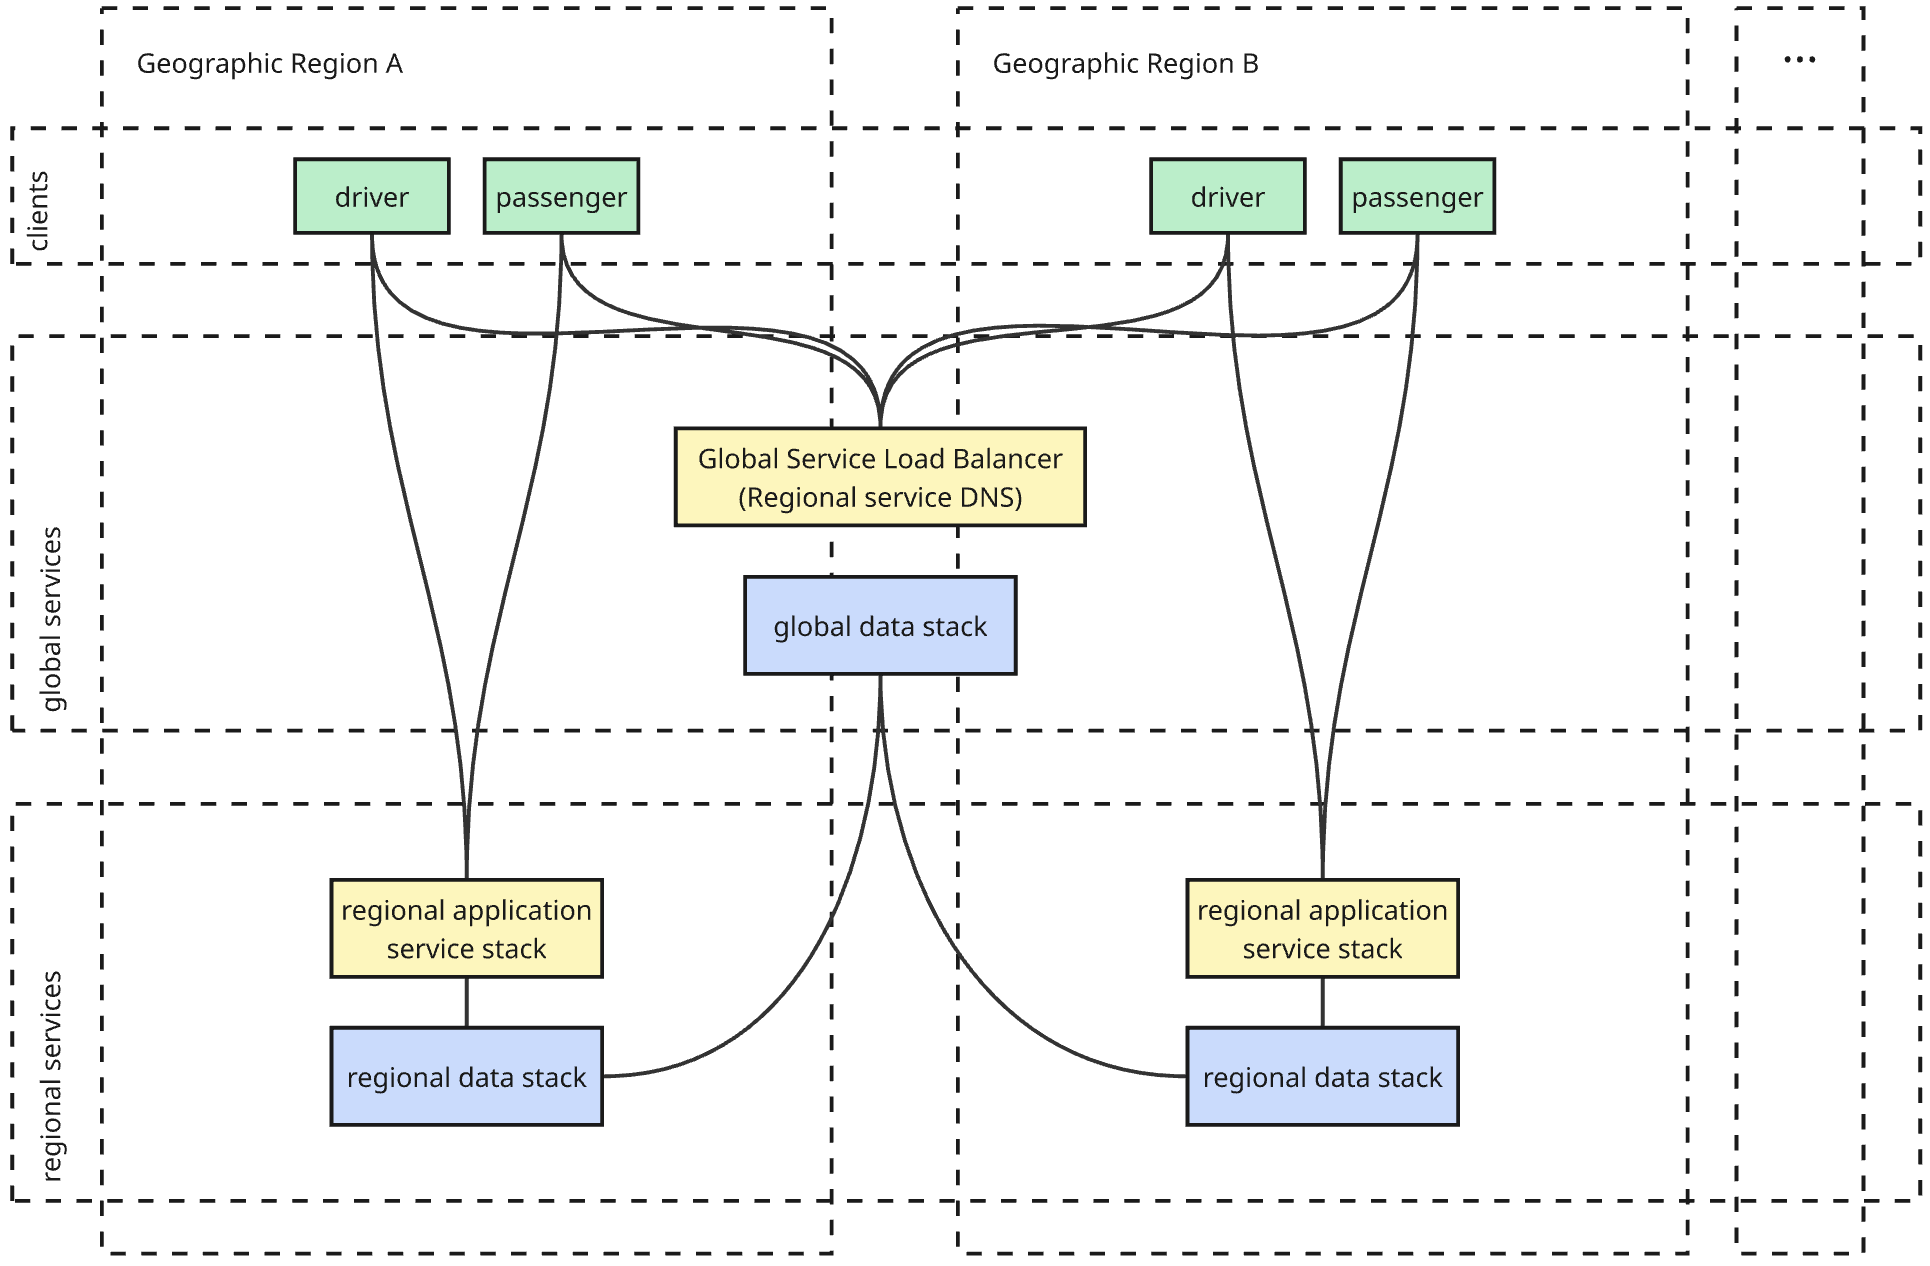
\includegraphics[width=0.9\textwidth]{architecture_overview.png}
    \caption{High-level system architecture.}
    \label{fig:architecture-overview}
\end{figure}

At the highest level the system components can be categorized into three groups: clients, global services, and regional services. The personas of the clients may be either passengers or drivers and their interfaces may be native mobile applications or web browsers. The global services are responsible for authentication, authorization, account management, and regional service routing. The bulk of core functionality is provided by the regional services, of which there can be an arbitrary number of instances.

When clients begin interacting with the system they query the global service load balancer (GSLB) to determine the appropriate regional service endpoint with which to communicate. The GSLB's DNS resolution is governed by a geolocation routing policy that maps a client's current IP address to a regional service gateway's IP address. This policy may also consider availability, capacity, and load.

\begin{figure}[H]
    \centering
    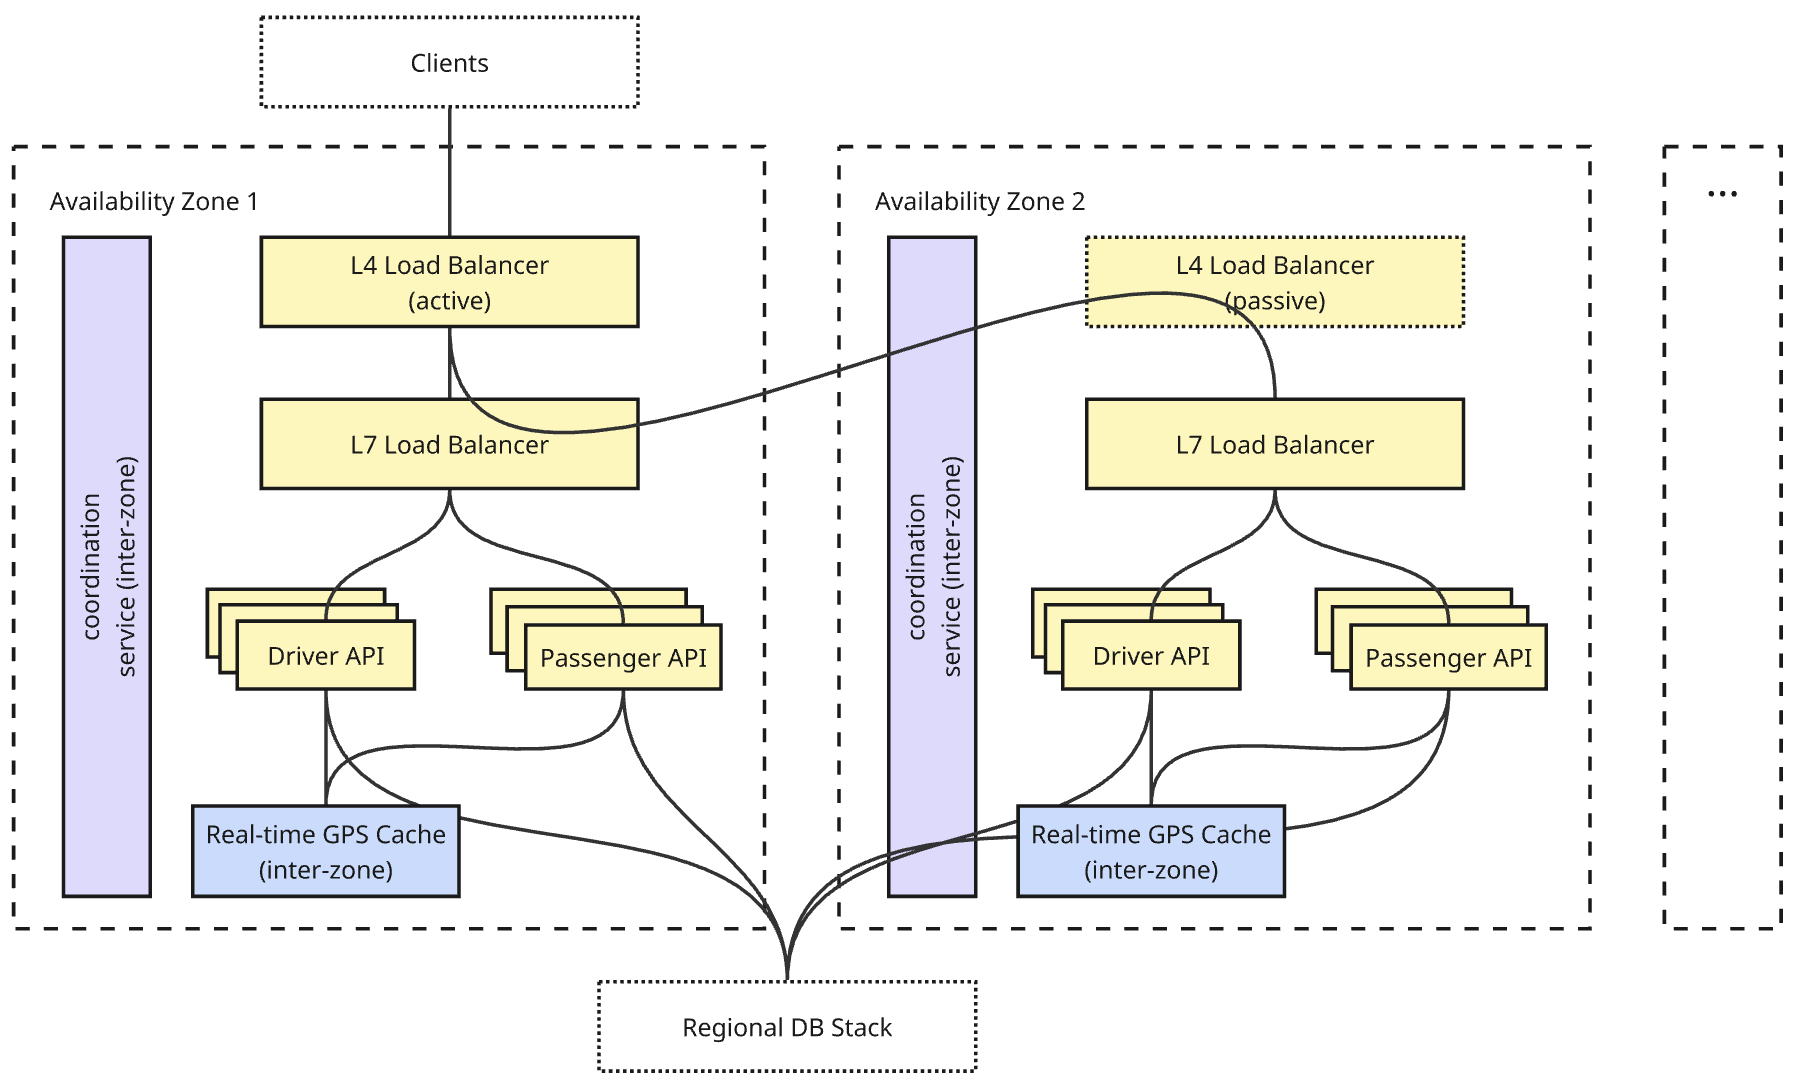
\includegraphics[width=0.9\textwidth]{regional_app_service_stack.png}
    \caption{Regional application service stack architecture.}
    \label{fig:regional-app-service-stack}
\end{figure}

Once a client has been routed to a regional service endpoint a layer 4 load balancer (L4LB) proxies their requests to an availability zone (AZ). The purpose of the L4LB is to distribute load across AZs and adapt to outages in AZs. At any given time there is a single active L4LB in a region, backed by instances that can take over should the active instance fail. Next, a layer 7 load balancer (L7LB) proxies requests to an appropriate application API based on the request path and headers. The L7LB is also responsible for TLS termination and rate limiting. This allows components deeper in the stack to focus on core functionality rather than security and load management.

Each application API can have multiple instances running, with the specific number scaling with the current or anticipated load. The API services are stateless which allows them to be regarded as ephemeral. The diagram depicts two specific APIs for illustration purposes, but in practice there will likely be many more along with additional supporting microservices. 
Each region also has an inter-zone distributed cache for rapidly changing non-durable data such as GPS locations of users. Durable data is managed by regional and global data stacks.
Finally, each region has a coordination service (CS) that spans AZs. The CS is responsible for leader election in the case of the L4LBs. It also provides service registration and discovery, enabling the L7LB to route to a flexible pool of API instances. 

Each regional data stack manages a distributed wide-column store cluster of high volume active ride data. Each cluster spans the AZs of its region, with peer nodes distributed across them. We use the H3 geospatial cell index as the partition key. The wide-column store distributes rows across nodes via consistent hashing with virtual nodes, which balances load evenly and minimizes data movement when the cluster is resized. Unlike a leader-follower database, the cluster is masterless: any node can accept reads and writes. Data is replicated to a configurable number of nodes per AZ for durability. Consistency is enforced at query time using a local quorum policy, requiring a majority of replicas within the region to acknowledge an operation before it is considered successful.

Applications are insulated from the complexity of the regional and global data stacks by a DB proxy (DBP). The DBP embeds a database driver that handles token-aware routing to the correct cluster node based on the partition key. The DBP's primary responsibilities are managing the connection pool and lazily loading records from the global data stack when new clients use the service or existing clients move between regions.

Each regional data stack has a coordination service used by the DBP for service discovery. Since the wide-column store cluster is masterless and uses gossip for internal node coordination, the CS is not involved in data node management. The DBP uses the CS to track which cluster nodes are healthy and should receive connections.

The global data stack is responsible for owning and managing durable data that is not specific to one single region. This data is much smaller in size and slower changing than the regional ride-based data, but arguably more critical to the system's operator: account information, payment information, and pricing rules for example. The global data stack is based around a single NewSQL cluster. This cluster has a number of replicated data nodes distributed across regions and AZs. This approach allows for quick reads and slow writes, which is fitting for the access pattern expected for this data. 

\subsection{Interaction Flows}

\begin{figure}[H]
    \centering
    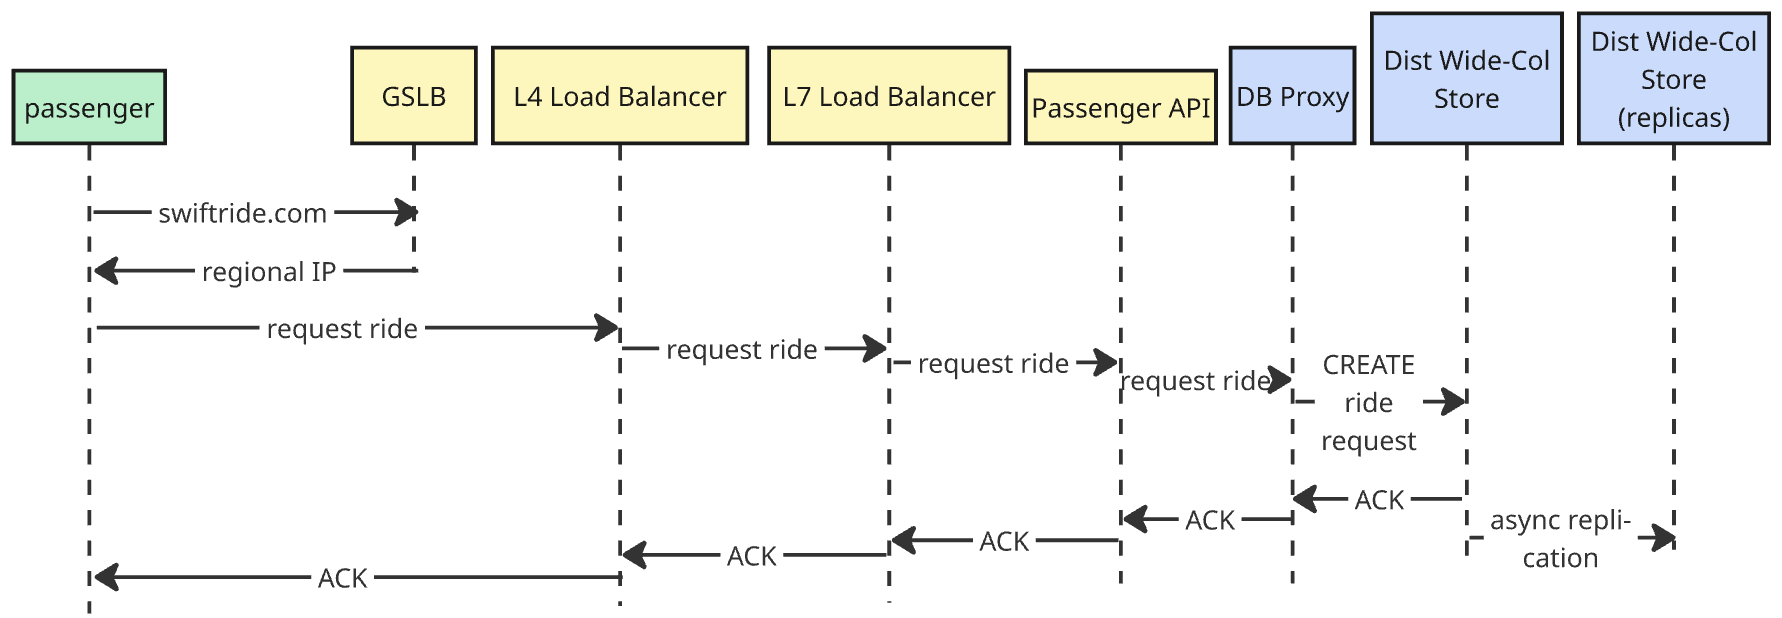
\includegraphics[width=0.9\textwidth]{ride_request.png}
    \caption{Ride request processing flow.}
    \label{fig:ride-request}
\end{figure}

The diagram traces a simplified ride request from a passenger. The full ride matching flow is more complex and is not shown in its entirety. A rider submits a trip request from their client. The request enters the regional stack through the L4LB and is routed by the L7LB to the ride matching service. The matching service executes a geospatial radius query against the GPS cache to identify available local drivers. From the candidates, the closest available driver is selected and tentatively assigned. The matching service then writes an active trip record to the wide-column store, recording the passenger, the driver, and the initial trip state. Once the write is acknowledged by a quorum, the driver is notified and the trip is live.

% ---------- Database Sharding ----------
\section{Database Sharding}
\label{sec:sharding}

\subsection{Sharding Strategies}

\subsubsection{Considered}
\begin{itemize}
    \item \textbf{Hash-based}: Assigns each record to a shard by hashing a key (e.g. user ID) and taking the result modulo the shard count. Writes spread evenly and routing is cheap to compute. However, adding or removing a shard changes the modulus, forcing a reshuffle of most existing data.
    \item \textbf{Range-based}: Assigns contiguous key ranges (e.g. timestamps) to specific shards. Range scans are cheap and the shard boundaries are easy to reason about, but it is susceptible to hotspotting. For example a single popular range, like downtown at rush hour, can lead to a single shard absorbing a disproportionate amount of the load. When a shard is removed, only its range needs to migrate to a neighboring shard. The rest of the dataset is untouched. The absorbing shard now owns a larger range, however, which can increase hotspot risk and may require a manual range split to rebalance.
    \item \textbf{Consistent hashing}\cite{consistenthashing}: Places shards and keys on the same hash ring, so adding or removing a shard only remaps the keys next to it on the ring rather than the whole dataset. It can still hotspot, since one shard may still own a disproportionate arc of the ring, but virtual nodes mitigate this by spreading each physical shard's ownership across many smaller arcs.
\end{itemize}

\subsubsection{Chosen}

The data in this system is partitioned at multiple levels. First, active ride data is isolated by region. We assume that regions have enough flexibility and scaling capacity that their count will rarely change. This is a form of range-based sharding where client IP addresses map to fixed regions. Second, within regional data stacks we shard data by geospatial index (H3\cite{h3}) using consistent hashing. This allows the number of shards to scale in response to demand without reshuffling the entire dataset, while also giving us shard keys that are semantically meaningful. As long as the granularity of the H3 cells is chosen appropriately, this approach will also avoid hotspotting. Range queries, such as finding all available drivers within a 2km radius, translate naturally to H3. Each cell has a defined area at a given resolution, so a radius query becomes a lookup over a small fixed set of neighboring cell IDs rather than a full scan.

% ---------- Replication and Consistency ----------
\section{Replication and Consistency Models}
\label{sec:replication-consistency}

\subsection{Consistency Model Comparison}

\subsubsection{Considered}
\begin{itemize}
    \item \textbf{Strong consistency}: All reads reflect the most recent write. Strong correctness guarantees and high latency
    \item \textbf{Eventual consistency}: Writes are acknowledged quickly and replicas converge over time. Reads may return stale data
    \item \textbf{Quorum-based consistency}: A write (or read) is acknowledged once a majority of replicas confirm it. A tunable hybrid of the preceding approaches.
\end{itemize}

\subsubsection{Chosen}

Each of these consistency models are represented in this system. We use quorum-based consistency for active trip data. A majority of replicas within the region must acknowledge a read or write before it is considered successful, giving us strong correctness guarantees without requiring cross-region coordination. We can accept the modest write latency cost because all replicas involved are within the same region.
The distributed GPS cache is eventually consistent, which is acceptable for data that is written frequently, read frequently, and does not involve accounting for real world resources: vehicles dispatched, rides cancelled, payment receipts, etc. Stale reads will not have a meaningfully negative impact on user experience. In return for the reduced consistency guarantee we get lower latency and very high throughput. This is ideal for the data that will be written orders of magnitude more often than other data types in the system.
Finally, we distinguish between two categories of global data. Security-critical user account fields (credentials, account status, payment methods, and driver approval status) require strong consistency globally. A deactivated driver who can still accept rides because a regional cache has not caught up is a safety issue, not a UX problem. These fields must always be read through to the global data stack, bypassing the regional DBP cache entirely. Profile data (display name, preferences, photo) can tolerate quorum-based consistency; stale reads have no meaningful consequence, and the latency cost of strong global consistency on every profile read is not justified.


% ---------- Load Balancing ----------
\section{Load Balancing}
\label{sec:load-balancing}

The system contains load balancers performing 3 distinct functions. The GSLB acts as a DNS resolver. Its only purpose is to direct clients to the correct region. It performs this task by mapping client IP addresses to fixed virtual IP (VIP) addresses used by L4LBs in each region. When a L4LB wants to move from passive to active it assumes the VIP.

L4LBs are the gateways for all inbound client traffic to each region. They act as true load balancers, distributing load across available downstream resources as efficiently as possible. They do not process requests or even investigate payloads. They operate at the level of the TCP protocol so the CPU usage is kept to a minimum.

Like the L4LBs, the L7LBs proxy requests towards application services, but L7LBs perform more middleware actions on the requests. Working at the HTTP/application level, these load balancers have access to request paths, methods, and headers. They use this information to filter, modify, and route requests to different types of APIs.


% ---------- Evaluation ----------
\section{Evaluation}

\subsection{Capacity and Latency}

\small
\begin{longtable}{@{}>{\raggedright\arraybackslash}p{2.3cm}>{\raggedright\arraybackslash}p{2.5cm}>{\raggedright\arraybackslash}p{2.8cm}>{\raggedright\arraybackslash}p{2.5cm}>{\raggedright\arraybackslash}p{4.5cm}@{}}
    \caption{Component throughput and latency BOTE estimates based on a survey of candidate implementations. Throughput values are given for a single instance of each component. Latency values are medians.}
    \label{tab:capacity}\\
    \toprule
    \textbf{Component} & \textbf{Technology} & \textbf{Throughput} & \textbf{Latency} & \textbf{Scaling}\\
    \midrule
    \endfirsthead
    \toprule
    \textbf{Component} & \textbf{Technology} & \textbf{Throughput} & \textbf{Latency} & \textbf{Scaling}\\
    \midrule
    \endhead
    \bottomrule
    \endlastfoot
    GSLB
        & DNS load balancer
        & $\sim$500K queries/s
        & $<$1ms
        & Horizontal with virtual IP \\
    \addlinespace
    L4LB
        & L4 load balancer
        & $\sim$200K connections/s
        & $<$1ms
        & Vertical. Horizontal with AZs \\
    \addlinespace
    L7LB
        & L7 load balancer
        & $\sim$100K req/s
        & 5ms
        & Vertical. Horizontal with AZs \\
    \addlinespace
    CS
        & Distributed coordination service
        & $\sim$50K ops/s \textit{(cluster)}
        & 10ms
        & Fixed (not directly impacted by load) \\
    \addlinespace
    DBP
        & Custom
        & $\sim$1M req/s
        & $<$1ms
        & Horizontal \\
    \addlinespace
    GPS Data Cache
        & Distributed key-value store
        & $\sim$1M ops/s
        & $<$1ms
        & Horizontal \\
    \addlinespace
    Active Trip Data
        & Distributed wide-column store
        & $\sim$100K writes/s
        & 5ms
        & Horizontal \\
    \addlinespace
    User Accounts
        & NewSQL database
        & $\sim$50K TPS
        & 100ms
        & Horizontal \\
    \addlinespace
    Trip History
        & Relational database
        & $\sim$50K reads/s
        & 10ms
        & Vertical for primary/write. Horizontal for reads \\
\end{longtable}
\normalsize

\subsection{CAP Theorem}

The CAP theorem\cite{captheorem} states that a distributed system can guarantee at most two of three properties:
\begin{itemize}
    \item \textbf{Consistency}: all nodes see the same data at the same time
    \item \textbf{Availability}: every request receives a response
    \item \textbf{Partition Tolerance}: the system continues operating despite network partitions
\end{itemize}

Since network partitions are a physical reality in any distributed system, partition tolerance is non-negotiable. The remaining choice is between consistency and availability when a partition occurs.

This system chooses CP vs. AP differently depending on data types. The GPS cache is AP. During a partition, nodes continue accepting reads and writes using whatever data they have. A driver's location being a few seconds stale does not affect safety or correctness. The matching process self-corrects on the next broadcast. Availability matters more here than precision.

The active trip data store is CP. We require local quorum acknowledgment before a write is considered successful. If a partition isolates enough replicas to break quorum, writes will fail rather than proceed with an inconsistent state. A conflict in trip state (e.g. two nodes believing different drivers are assigned to the same rider) is not recoverable and is far worse than a temporary write failure.

The global user account store is also CP. Security-critical fields such as account status, credentials, and payment methods must be consistent everywhere before a change is readable. A deactivated driver account that remains active in a partitioned region is a safety issue. We accept that writes to these fields may be rejected during a global partition rather than risk allowing stale reads.

\section{Technology Recommendations}
\label{sec:technology-recommendations}

Thus far the system has been described in terms hardware and software agnostic to the extent possible. The system as-is can be implemented with various technologies. In the process of selecting specific environments and frameworks, some singular components may split into multiple, while others may be combined. What follows is an exercise that illustrates how this system might be implemented.

We have chosen to use open-source technologies where possible, to avoid vendor lock-in and to allow for greater flexibility in deployment. The following table summarizes the software recommendations for each system component, along with rationale for each.

\subsection{Infrastructure}
We will use a cloud provider for the underlying physical infrastructure. This allows us to get up and running quickly with the ability to scale along the way. The specific provider is not important as no provider specific services will be used. (In reality, this may not be the best decision. This was done to allow for learning about open source technologies.)

The compute and networking resources needed to run the system will be provisioned with Terraform. After provisioning, the system will be deployed and configured with Ansible. These two tools allow us to define the system architecture with code instead of manually standing up the infrastructure: it's fast, readable, and repeatable.

The app services (e.g. APIs) will require more active management than Ansible is intended to provide. There we will containerize the services and mange the containers with Kubernetes \cite{kubernetes}. Kubernetes can be configured to automatically scale with load and we also get metrics and logging out of the box.

\subsection{Software}

\small
\begin{longtable}{@{}>{\raggedright\arraybackslash}p{3.3cm}>{\raggedright\arraybackslash}p{3.6cm}>{\raggedright\arraybackslash}p{8.8cm}@{}}
    \caption{Software recommendations by system component.}
    \label{tab:tech-recommendations}\\
    \toprule
    \textbf{Component} & \textbf{Recommendation} & \textbf{Rationale}\\
    \midrule
    \endfirsthead
    \toprule
    \textbf{Component} & \textbf{Recommendation} & \textbf{Rationale}\\
    \midrule
    \endhead
    \bottomrule
    \endlastfoot
    GSLB
        & PowerDNS \cite{powerdns}
        & Supports geolocation-based DNS resolution and health-check-driven failover \\
    \addlinespace
    L4LB
        & HAProxy \cite{haproxy}
        & High-throughput TCP proxy with active/passive failover. Adds negligible latency. \\
    \addlinespace
    L7LB
        & Envoy \cite{envoy}
        & Path and header-based routing, TLS termination, rate limiting, and built-in observability. \\
    \addlinespace
    CS
        & etcd \cite{etcd}
        & Raft-based consensus purpose-built for leader election and service discovery. Proven at scale. \\
    \addlinespace
    DBP
        & Custom service
        & H3 token-aware routing, shard discovery via the CS, and lazy cross-region loading are all app-specific. No DB proxy handles this combination out-of-the-box. \\
    \addlinespace
    GPS Data
        & Redis \cite{redis}
        & Supports geospatial commands (\texttt{GEOADD}, \texttt{GEORADIUS}) and per-key TTL. Sub-millisecond latency at high write volume. \\
    \addlinespace
    Pricing Rules
        & Redis
        & Fits entirely in memory. Replication provides regional availability; TTL invalidation handles infrequent updates. \\
    \addlinespace
    Active Trip Data
        & Apache Cassandra \cite{apachecassandra}
        & Masterless, horizontally scalable across AZs. Tunable consistency supports the local quorum policy chosen for trip records. \\
    \addlinespace
    User Accounts
        & CockroachDB \cite{cockroachdb}
        & Serializable isolation satisfies the strong consistency requirement. Geo-partitioning anchors records to their home region for fast local reads. \\
    \addlinespace
    Trip History
        & PostgreSQL \cite{postgresql}
        & Time-based range partitioning aligns directly with the sharding strategy for this data. Mature SQL covers the analytical and auditing queries expected here. \\
\end{longtable}
\normalsize

% ---------- References ----------
\bibliographystyle{plain}
\bibliography{references}

\end{document}
